\documentclass[10pt,hyperref={CJKbookmarks=true},xcolor=dvipsnames,aspectratio=169]{beamer}
\usetheme[navigation]{UMONS}
\usepackage[utf8]{inputenc}
\usepackage{verbatim}
\usepackage{ctex}

\title[国际经济学]{国际经济学}
    \subtitle{Introduction}
	\author{鲁晓东}
\institute[]{%
	岭南学院\hspace{2em}中山大学
	\\[4ex]
  
\includegraphics[height=8ex]{fig/lingnanlogo}\hspace{2em}%

\includegraphics[height=8.5ex]{fig/sysu}
}

\begin{document}
\maketitle


\begin{frame}
\frametitle{提纲}
\tableofcontents
\end{frame}				%生成提纲页

%-----------正文开始----------------------

\section[Introduction]{Introduction}

\begin{frame}{What's International Trade About?}




\begin{itemize}
	\item Do you have any expectation for this course?
	\item 迄今,你认为2018年经济领域发生的最significant的事是什么?
	\item 如果你想赢,你必须先知道它是如何运作的
\end{itemize}
\begin{block}{2017年中国贸易情况}
	2017年,中国\textbf{货物贸易总额27.79万亿人民币},折合\textbf{4.105万亿美元}。其中,出口15.33万亿元,增长10.8\%;进口12.46万亿美元,增长20.9\%;贸易顺差2.87万亿美元,收窄14.2\%;\\
	2017年,中国前三大贸易伙伴分别是\textbf{欧盟、美国和东盟},三者合计占我国进出口总值的41.8\%;\\
	2017年,中国\textbf{一般贸易}进出口15.66万亿元,占比56.4\%,贸易结构有所优化;\\
	2017年,中国出口最多的产品是\textbf{机电类产品},共出口8.95万亿,占比58.4\%,传统劳动密集型产品合计出口3.08万亿元,占比21.1\%;进口最多的三类商品是原油、铁矿石,汽车。\\
\end{block}
\end{frame}

\begin{frame}

\begin{columns}[onlytextwidth]
	\begin{column}{0.45\textwidth}
		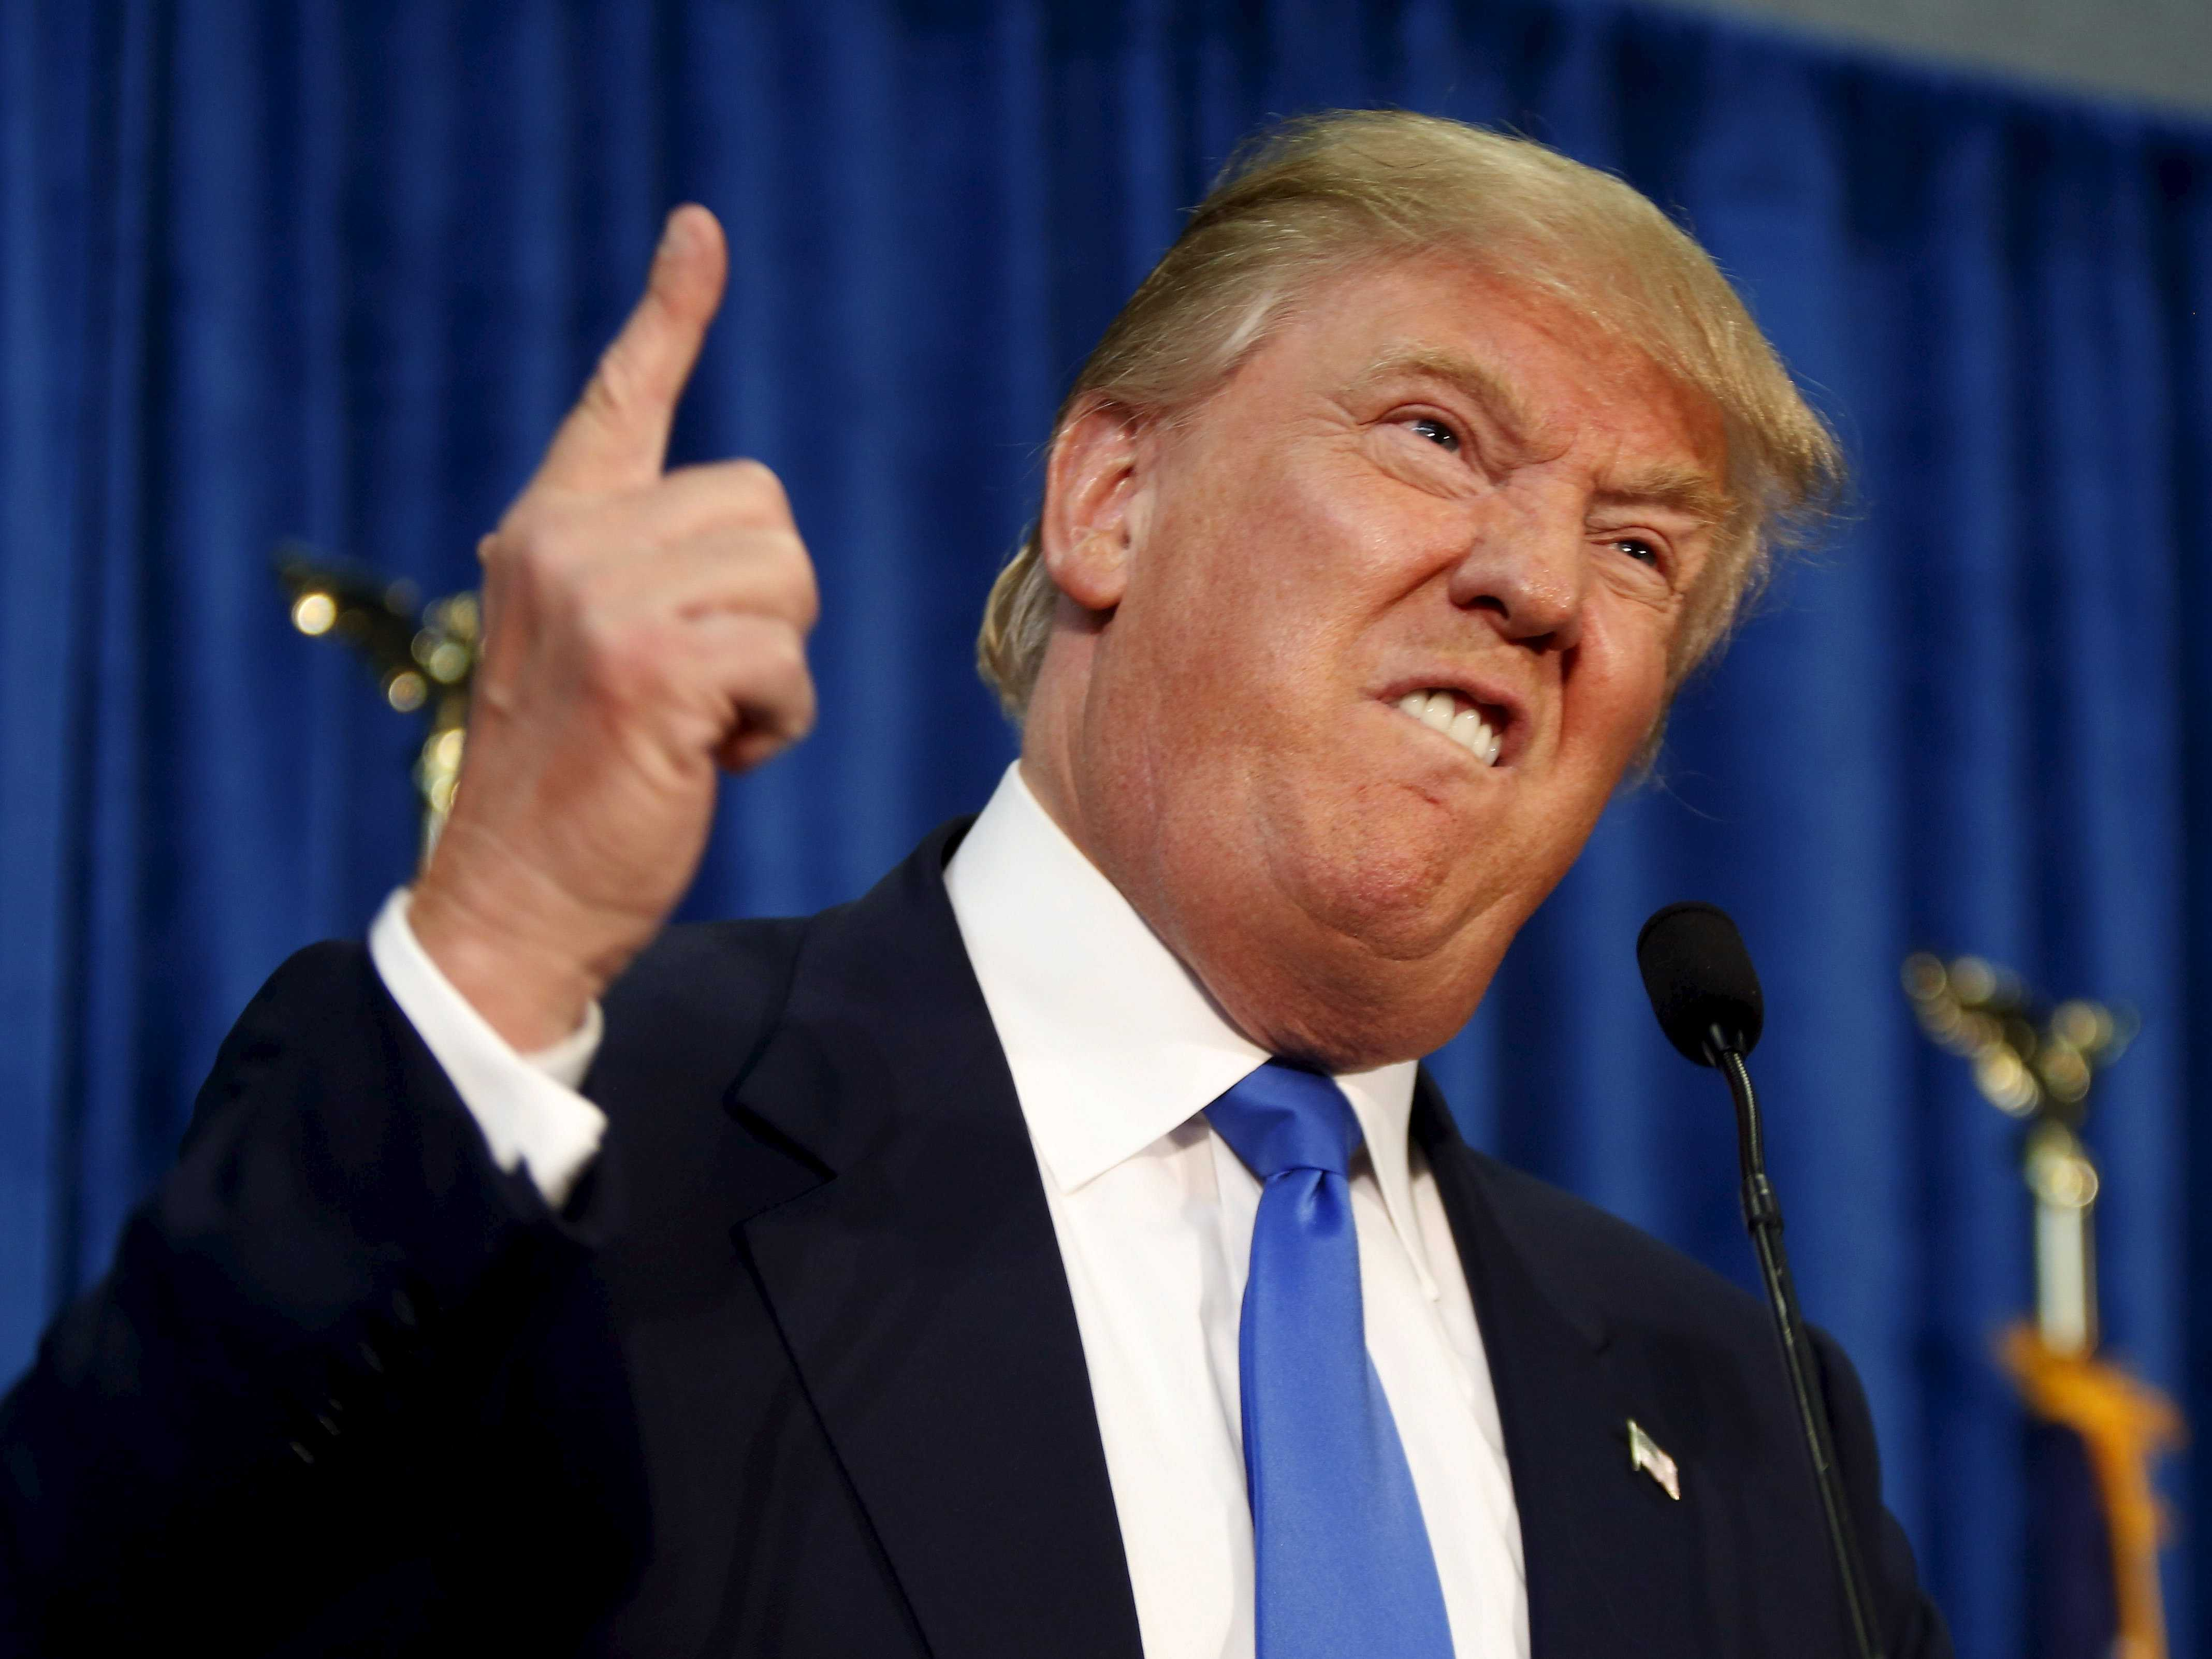
\includegraphics[width=\columnwidth]{fig//trump}
	\end{column}
	\begin{column}{0.55\textwidth}
		
		
		\begin{itemize}
			\item Who is this Guy?
			
			\begin{itemize}
				\item The enemy of free trade
				\item What's his opinion and policy on trade?
				\item Does that make sense?
			\end{itemize}
		\end{itemize}
	\end{column}
\end{columns}
\end{frame}

\begin{frame}{What's the direct of impact of Trump's trade war with China}


\begin{figure}
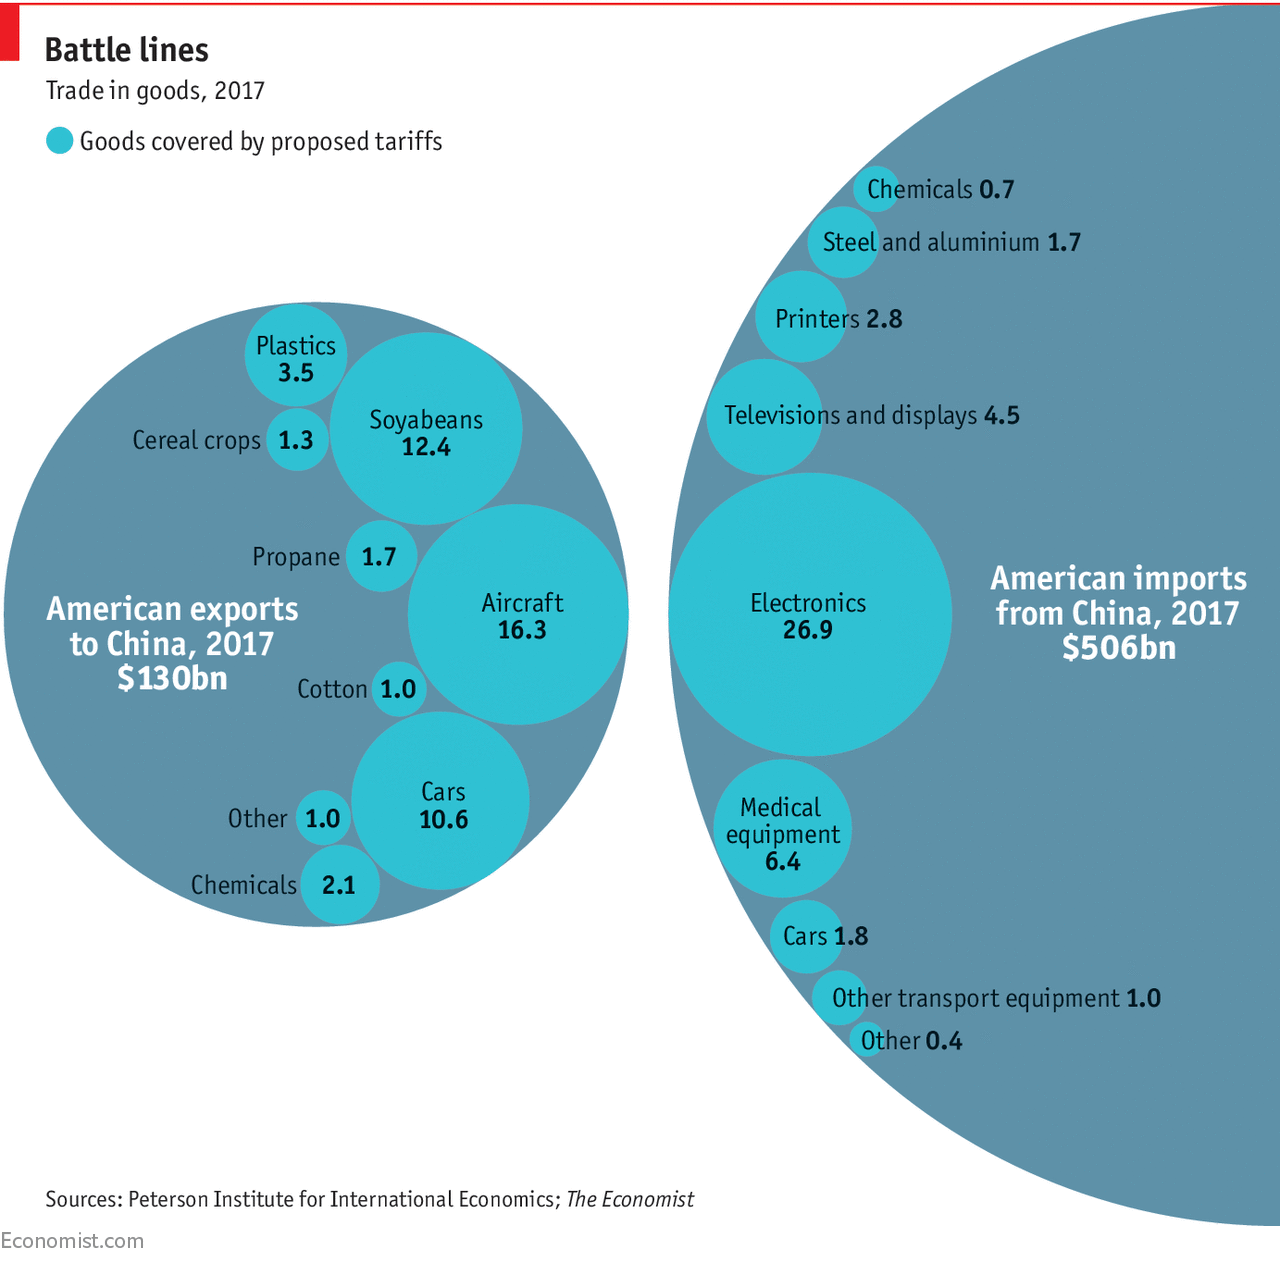
\includegraphics[scale=0.15]{fig//trump2.png}

\end{figure}

\end{frame}

\begin{frame}{Is WTO a total disaster for America?}

\begin{itemize}
\item What is NAFTA/WTO?
\item Does China (or Free Trade) steal manufacturing jobs from America?
\begin{figure}


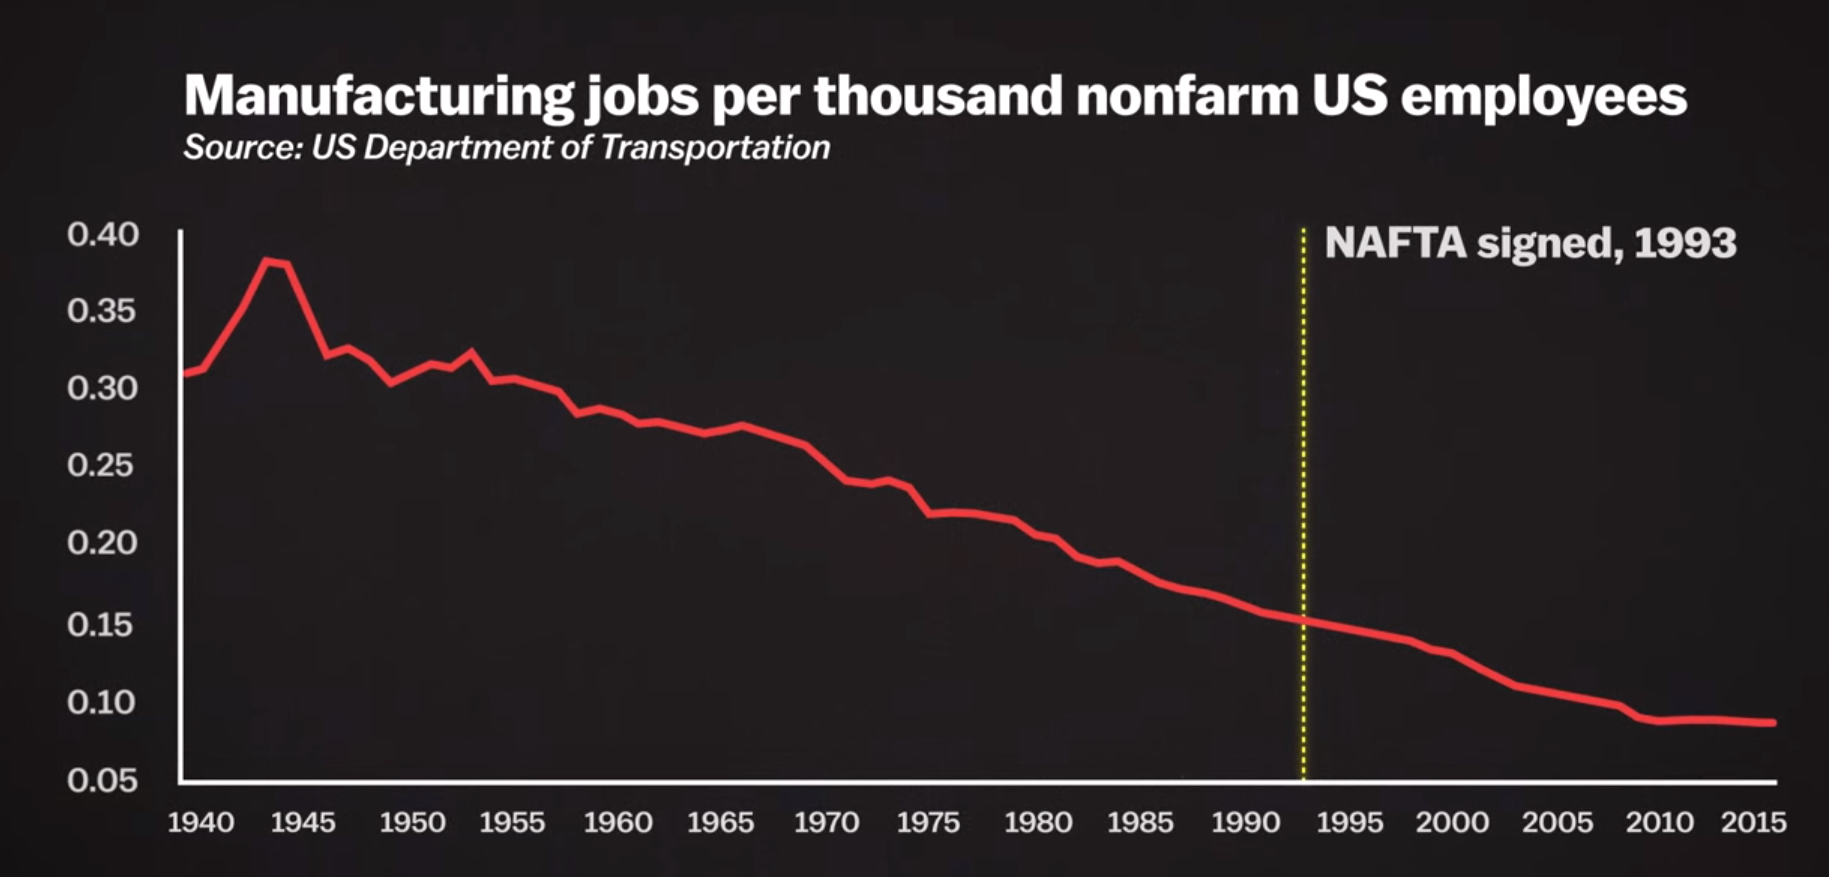
\includegraphics[scale=0.2]{fig//trump3}

\end{figure}

\end{itemize}
\end{frame}

\begin{frame}{Besides this, Trump have quit TPP}


\begin{columns}[onlytextwidth]
\begin{column}{0.4\textwidth}
\begin{itemize}
\item What is TPP?
\item Is it really a good thing to America?
\end{itemize}

\end{column}
\begin{column}{0.6\textwidth}
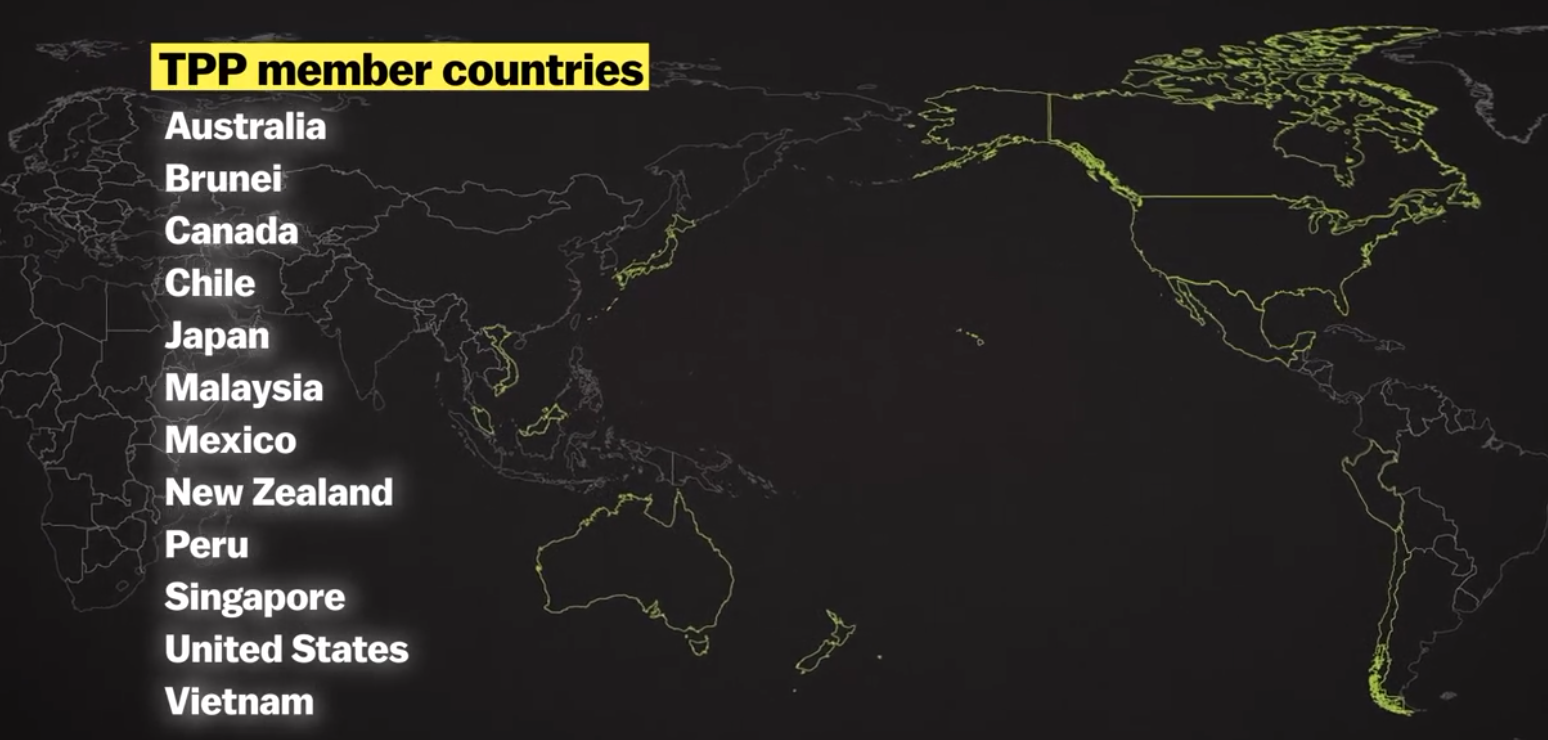
\includegraphics[width=\columnwidth]{fig//trump4}
\end{column}
\end{columns}

\end{frame}

\begin{frame}{Who would be the loser of exiting TPP?}


\begin{columns}[onlytextwidth]
\begin{column}{0.45\textwidth}
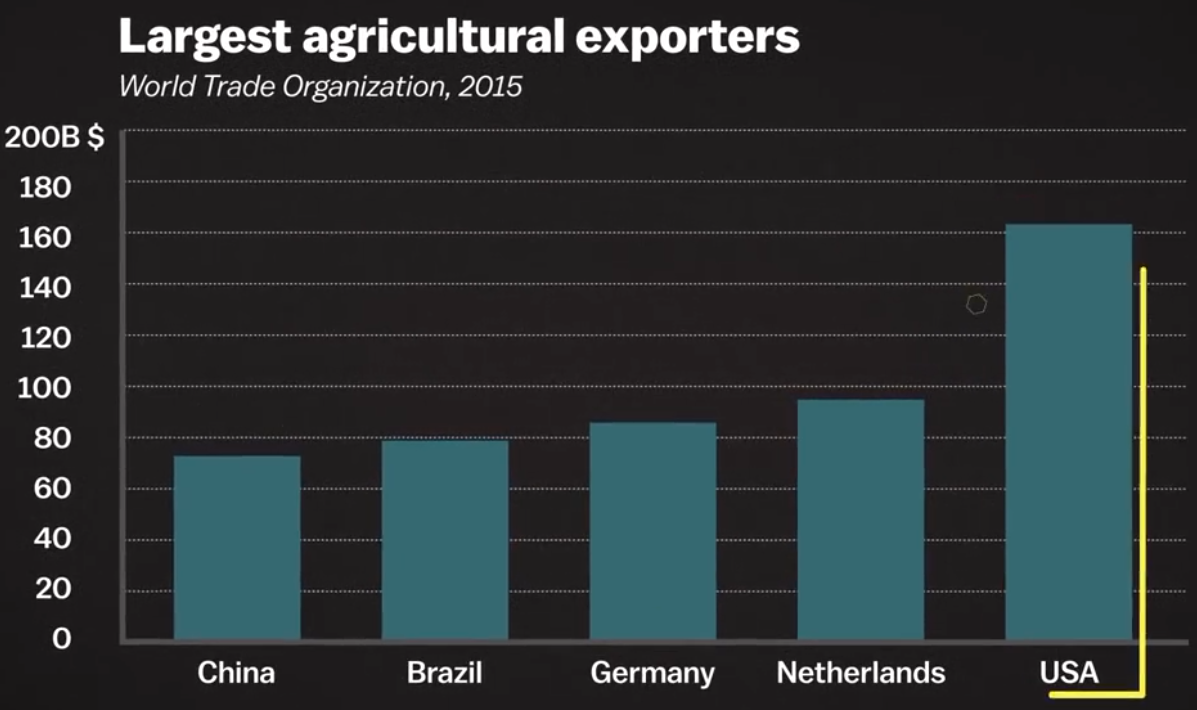
\includegraphics[width=\columnwidth]{fig//trump6}
\end{column}
\begin{column}{0.45\textwidth}
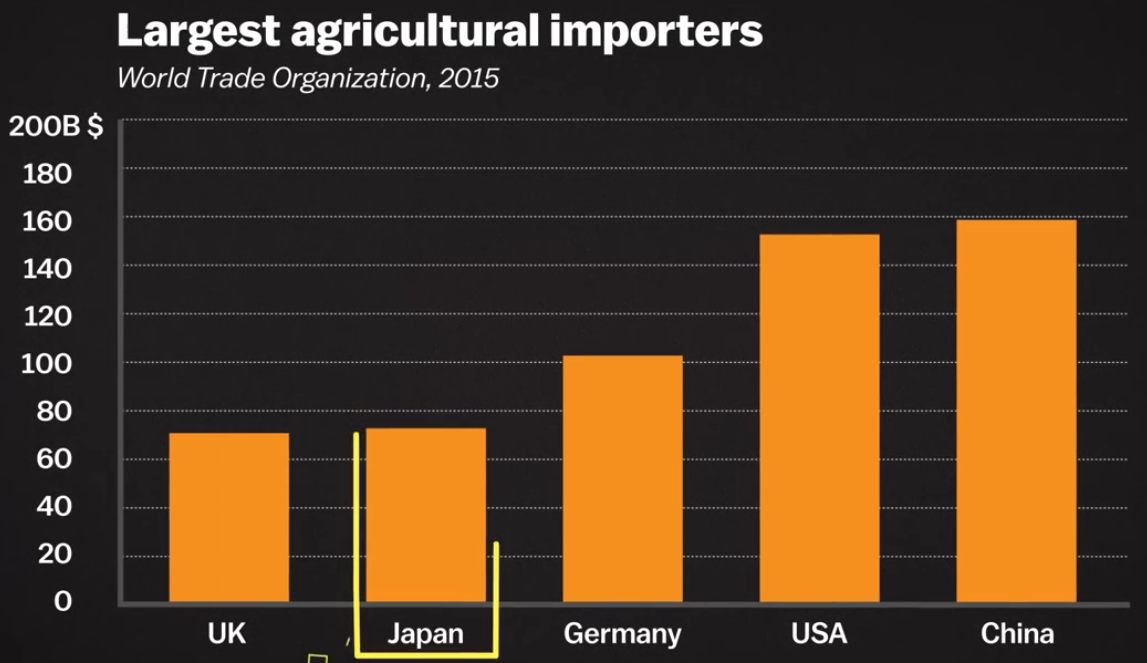
\includegraphics[width=\columnwidth]{fig//trump7}
\end{column}
\end{columns}
\end{frame}

\begin{frame}{Is this an opportunity to China}


\begin{columns}[onlytextwidth]
\begin{column}{0.4\textwidth}
\begin{itemize}
\item What is the role of China in the world trade map?
\item Obs, China now become the advocator of free trade and defender of
globalizaiton, Does that mean China would and could be the leader
of world trade?
\end{itemize}

\end{column}
\begin{column}{0.6\textwidth}
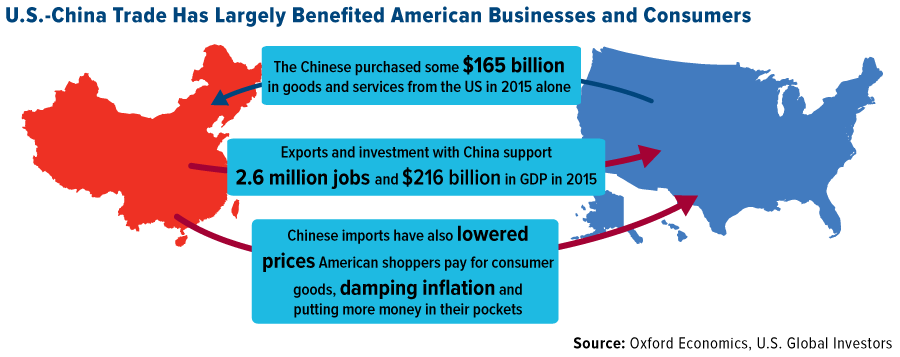
\includegraphics[width=\columnwidth]{fig//trump5}
\end{column}
\end{columns}

\end{frame}

\section{Administrative Stuff}
\begin{frame}{Missions of the course}

\begin{itemize}
\item 现实takeaways
\begin{itemize}


\item Teaches you something that the president will never understand
\item Provides you the truth behind trade war, 离真理近一些,离盲从远一点

\item inspire to think the benefits of trade
\item unfolds how the world trade is operating
\end{itemize}
\item 理论(经济学)takeaways
\begin{itemize}

\item tracks down the source of economics where it is initiated
\item tells you the great insight and talence created by great economists,
including their gossip
\item reveals how economics would be extended in the context of open ecnomy
\end{itemize}

\end{itemize}
\end{frame}

\begin{frame}{Highlights of the Syllabus}


\begin{columns}[onlytextwidth]
\begin{column}{0.55\textwidth}
\begin{itemize}
\item Required Textbook:

\begin{itemize}
\item Paul Krugman and Maurice Obstfeld, International Economics: Theory
and Policy, 8th edition, Published by PEARSON EDUCATION LTD.
\item Robert C Feenstra, Alan M Taylor, International Macroeconomics, 2e,
Worth Publishers, New York and Basingstoke
\end{itemize}
\item Many other readings in the Syllabus, but only recommended (not required) 
\end{itemize}

\end{column}
\begin{column}{0.35\textwidth}
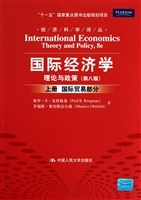
\includegraphics[scale=1]{fig//krugman_textbook}
\end{column}
\end{columns}

\end{frame}






\begin{frame}{Grading Policy}

\begin{itemize}
\item Participation \structure{\textcolor{red}{10\%}}
\item Homework \structure{\textcolor{red}{20\%}}

\begin{itemize}
\item Six problem sets will be distributed during the semester. These problem
sets will be collected and evaluated, and answers will be posted on
the course online platform (\textcolor{red}{ftp.lingnan.net, id \&
pw: luxd}).
\end{itemize}
\item Final exam \structure{\textcolor{red}{70\%}}

\begin{itemize}
\item The exam will cover information provided by lectures, readings, online
and in-class discussions. It will be close to book and related notes. 
\end{itemize}
\item Term Paper-\emph{Optional}

\begin{itemize}
\item I am open to the possibility of a term paper in case you would like
to use the knowledge and tools in this course to complete your research.
\end{itemize}
\end{itemize}
\end{frame}

\begin{frame}{How to Reach Me}


\textbf{Instructor:Dr. Lu Xiaodong}
\begin{itemize}
\item Department of Economics, Associate professor
\item luxiaod@mail.sysu.edu.cn 
\item Office Hours: Room511, S. J. Wong Hall, 
\item Lecture Time: Thursday 8:55-11:30am
\end{itemize}


\textbf{TA: TBA}
\end{frame}

\begin{frame}{Goal and Approach for the Class}

\begin{itemize}
\item \textbf{Goal:} Be able to understand and analyze past and current
events in the world economy on your own
\item \textbf{Approach:} Will rely on formal modeling techniques to achieve
this goal
\begin{itemize}
\item You must be very comfortable with the course of Principle of Economics,
especially Microeconomics
\item Course is not mathematically demanding, but the concepts studied are
not trivial and require careful formalization 
\item I will do my best to motivate the models with specific \structure{examples}
\end{itemize}
\end{itemize}
\end{frame}

\section{Whole Story of IE}%
\begin{frame}{What is International Economics About}

\begin{itemize}
\item Is there any stuffs that can be transfered acorss the border of one country?
\item International economics studies the \structure{exchange of goods and services} and corresponding flows of capital  \structure{across international boundaries or territories} 

\end{itemize}

\end{frame}


\begin{frame}{General Course Outline\\International Trade}

\begin{enumerate}
\item Trade volume and its determinations
\begin{enumerate}
\item Volume of Trade: Why we trade So much(small)?	 	
\end{enumerate}
\item Trade pattern and its determinations
\begin{enumerate}
\item Trade and Technology: The Ricardian Model 
\item Gains and Losses from Trade in the Specific-Factors Model 
\item Trade and Resources: The Heckscher-Ohlin Model 
\item Movement of Labor and Capital between Countries 
\item Increasing Returns to Scale and Monopolistic Competition. 
\item Multinational Firm: Offshoring of Goods and Services 
\end{enumerate}
\item International Trade Policy
\begin{enumerate}
\item Instruments to influence trade flow
\item Welfare effect of trade policy
\item International trade coordination: WTO
\item International trade coordination: RTA
\end{enumerate}
\end{enumerate}
\end{frame}

\begin{frame}{General Course Outline-International Finance}

\begin{enumerate}
	\item 汇率市场与汇率理论 
		\begin{enumerate}
			\item 汇率与外汇市场
			\item 长期汇率理论
			\item 短期汇率理论
		\end{enumerate}

	\item 国际收支 
		\begin{enumerate}
			\item 国际收支平衡表与开放条件下的国民经济核算
			\item 国际收支理论
		\end{enumerate}

	\item 国际货币体系 
		\begin{enumerate}
			\item 国际货币体系演变
			\item 汇率制度选择
			\item 货币危机
			\item 最优货币区理论与欧元
			\item 债务危机
		\end{enumerate}

\end{enumerate}
\end{frame}



\end{document}